\documentclass[Visionprosjekt.tex]{subfiles}
\NormalTopp
\begin{document}

%%%%%%%%%%%%%%%%%%%%%%%%%%%%%%%%%%%%%%%%%%%%%%%%
\section{Vision}
%%%%%%%%%%%%%%%%%%%%%%%%%%%%%%%%%%%%%%%%%%%%%%%%
Maskiner som kan "<se">, kan inspisere produkter etter defekter, ta mål, lese strekkoder og lignende. \red{Ja, hva med slike maskiner? TULLESETNING!} Maskinen innhenter informasjon fra kameraet og behandler den etter forhåndsbestemte, egendefinerte regler. I sin enkleste form består et digitalt kamera av et objektiv, en bildebrikke, rådata bildebehandler, og en lystett kapsling. Bildebrikka har tusenvis av små lysfølsomme punkter eller pixler, og objektivet vil, med korrrekt justert fokus, tegne et bilde på bildebrikka. Se \reff{fig:kamera} for en illustrasjon for et kameras virkemåte. For kamera som er brukt i dette prosjektet vil hvert enkelt punkt på bildebrikka overføre en verdi mellom 0 og 255 som forteller hvor mye lysintensiteten på det enkelte punkt. Disse verdiene blir normalisert til verdier mellom 0 og 100 i bildebehandlingsdelen i kamera.

\begin{figure}[ht]
	\centering
		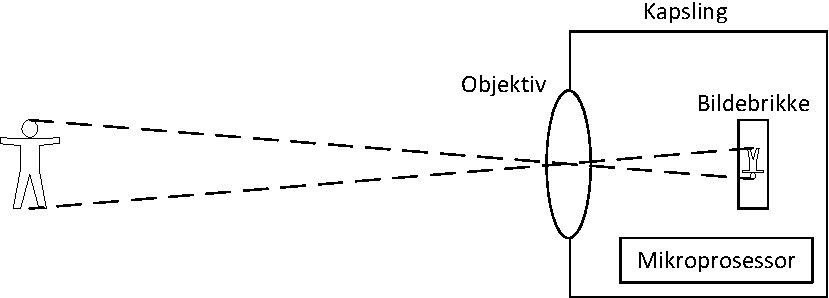
\includegraphics{bilder/kamera}
	\caption{Virkemåte av et kamera}
    \label{fig:kamera}
\end{figure}


%%%%%%%%%%%%%%%%%%%%%%%%%%%%%%%%
\subsection{Beskrivelse}
%%%%%%%%%%%%%%%%%%%%%%%%%%%%%%%%
Visionsystemet består av en I/O-modul med utvidelsesspor i tillegg til kamera. Kameraet har en innebygget bildeanalysator som heter "<SmartImage Sensor">. Det er bildeanalysatoren som er selve hjernen til kameraet, og analyserer bildet etter de forhåndsdefinerte reglene. På bildeanalysatoren kjører en programvare som heter "<FrameWork Firmware">, \red{og programversjonsnummeret må være lik den som brukes til programmering på PC.}




%%%%%%%%%%%%%%%%%%%%%%%%%%%%%%%%
\subsection{Spesifikasjoner}
%%%%%%%%%%%%%%%%%%%%%%%%%%%%%%%%
Se \reft{tab:legend530} for spesifikasjoner for kameraet DVT Legend 530 \cite{dvtlegend530}.

\begin{table}[ht]
    \centering
    \caption{Spesifikasjoner for DVT Legend 530}
    \label{tab:legend530}
    \begin{tabularx}{0.65\textwidth}{lX}
    \toprule
        Egenskap        &   Verdi\\
    \midrule
        Bildebrikke	    &	4.8\,mm $\times$ 3.6\,mm CCD\\
        Oppløsning	    &	640\,px $\times$ 480\,px gråskala\\
        Strømtilførsel	&	24\,VDC 210 mA\\
        Temperaturområde i drift	&	0--45\,°C\\
        Objektivfeste	&	CS-feste\\
        Ekstrautstyr	&	LED-belysning\\
        \bottomrule
    \end{tabularx}
\end{table}

Det er tilgang på to objektiver for kameraet. Hovedforskjellen er fokuslengden. Se \reft{tab:objektiver} for spesifikasjoner for objektivene.



\begin{table}[ht]
    \centering
    \caption{Spesifikasjoner for objektivene}
    \label{tab:objektiver}
    \begin{tabularx}{0.65\textwidth}{llX}
        \toprule
         Egenskap               &	6\,mm f/1.4	&	Tamron 16\,mm f/1.4\\
        \midrule
        Feste	                &	C-feste	    &	C-feste\\
        Fokuslengde	            &	6\,mm	    &	16\,mm\\
        Største blenderåpning	&	f/1.4	    &	f/1.4\\
        Minste blenderåpning	&	Stengt	    &	f/16\\
        Nærgrense	            &	20\,cm	    &	30\,cm\\
        \bottomrule
    \end{tabularx}
\end{table}


CS-festet har en FFD, Flange Focal Distance, på 12.526\,mm. C-feste har en FFD på 17.526\,mm \cite{CSmount}. Det betyr at det må settes inn en 5\,mm fokusforlenger. En slik fokusforlenger er det tilgang på. Under prøving av kamera og objektiv fungerte ikke fokusforlengeren som tiltenkt, og det måtte lages en 1\,mm tykk skive til å flytte FFD til 18.526\,mm. Dette gjorde at nærgrensen til objektivet ble lavere, som betyr at kamera kan settes enda nærmere objektene som skal fotograferes.

\end{document}